\documentclass[varwidth,convert={density=500,outext=.png},border=0pt]{standalone}

% Tikz packages
\usepackage{tikz}
\usetikzlibrary{%
  patterns, plotmarks, backgrounds, shapes, arrows, calc, trees, positioning,
  chains, shapes.geometric, decorations.pathreplacing,
  decorations.pathmorphing, shapes.arrows, decorations.markings, quotes,
  arrows.meta, spy, fit, matrix
}

% General includegraphics and colour support
\usepackage{graphicx}
\usepackage{xcolor}
% Captions and subcaptions
\usepackage{caption}
\usepackage[labelformat=parens]{subcaption}

% String macros (for reading in tabular data)
\usepackage{xstring}

% PGFPlots
\usepackage{pgfplots}
\usepackage{pgfplotstable}
\pgfplotsset{compat=newest,plot coordinates/math parser=false}

%% Define node types
\tikzstyle{lnode} = [%
  circle,
  draw=black,
  minimum height=1.3cm,
  align=center,
  fill=none,
  text centered,
  inner sep=0.5pt,
  font=\tiny
]%
\tikzstyle{rxn} = [%
  rectangle,
  draw=black,
  minimum width=0.3cm,
  minimum height=0.3cm,
  align=center,
  fill=none,
  text centered,
  inner sep=0.5pt,
  font=\tiny
]%

\begin{document}
  \begin{figure}
    \centering
    \scalebox{0.75}{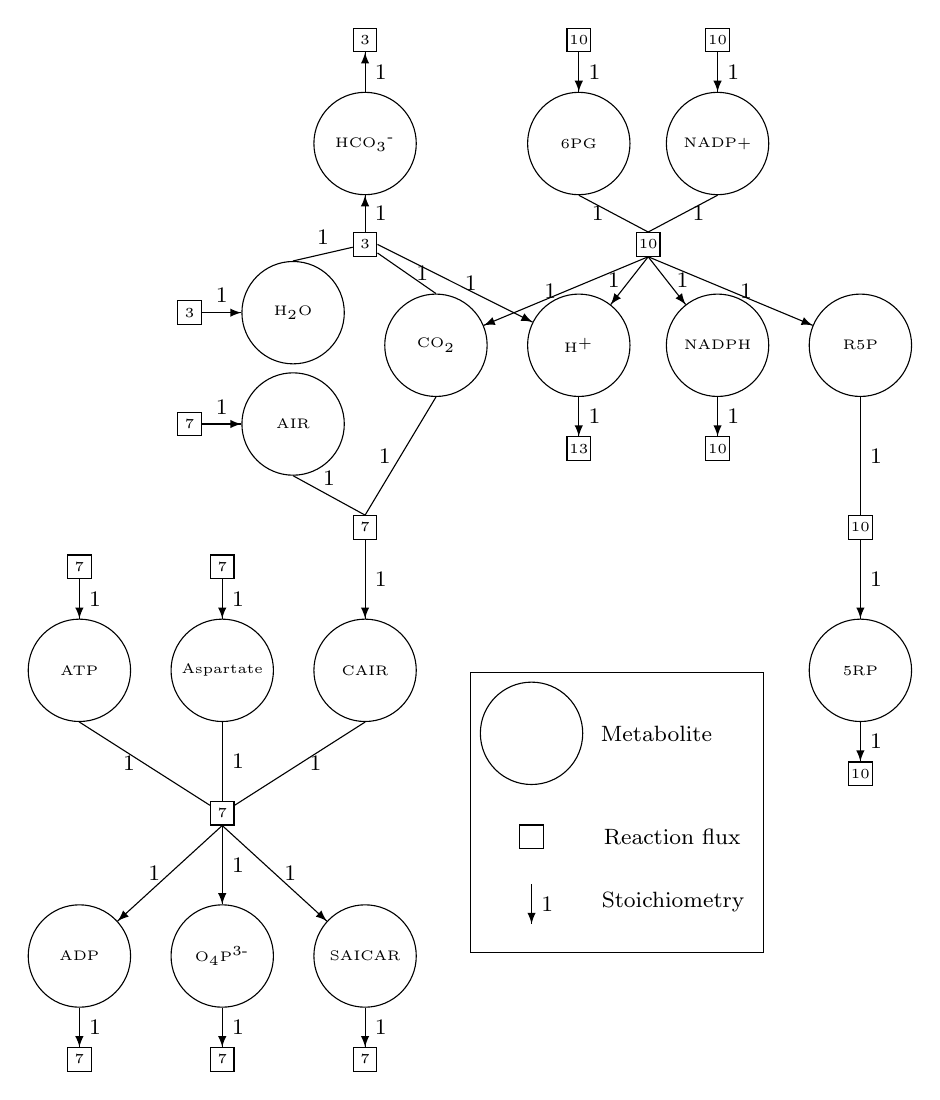
\begin{tikzpicture}[%
  >=latex,
  decoration={%
    markings,
    mark=at position 1.0 with {\arrow{>}}
  },
  every node/.style={%
    %font=\sffamily\footnotesize\itshape,
    font=\footnotesize,
    text=black,
    text centered,
    align=center
  },
  frame/.style={draw=black,inner sep=2pt}
]

  % Nodes
  \node[] (P1) {};
  \node[lnode,text=black,left=0.1cm of P1] (A1) {6PG};
  \node[lnode,text=black,right=0.1cm of P1] (A2) {NADP+};
  \node[rxn,below=1.0cm of P1] (R1_2) {10};
  \node[below=1.0cm of R1_2] (P2) {};
  \node[lnode,text=black,left=0.1cm of P2] (A4) {H\textsuperscript{+}};
  \node[lnode,text=black,right=0.1cm of P2] (A5) {NADPH};
  \node[lnode,text=black,right=0.5cm of A5] (A6) {R5P};
  \node[rxn,text=black,below=1.5cm of A6] (R6) {10};
  \node[lnode,text=black,below=1.0cm of R6] (A7) {5RP};
  \node[lnode,text=black,left=0.5cm of A4] (A3) {CO\textsubscript{2}};
  \node[lnode,text=black,left=0.5cm of A3,yshift=-1.0cm] (A8) {AIR};
  \node[lnode,text=black,above=0.1cm of A8] (A15) {H\textsubscript{2}O};
  \node[rxn,xshift=-0.9cm] (R3_15) at (A3 |- R1_2) {3};
  \node[lnode,text=black] (A16) at (A1-|R3_15) {HCO\textsubscript{3}\textsuperscript{-}};
  \node[rxn] (R3_8) at (R6-|R3_15) {7};
  \node[lnode,text=black,below=1.0cm of R3_8] (A9) {CAIR};
  \node[lnode,text=black,left=0.5cm of A9] (A10) {Aspartate};
  \node[lnode,text=black,left=0.5cm of A10] (A11) {ATP};
  \node[rxn,text=black,below=1.0cm of A10] (R9_10_11) {7};
  \node[lnode,text=black,below=1.0cm of R9_10_11] (A13) {O\textsubscript{4}P\textsuperscript{3-}};
  \node[lnode,text=black,left=0.5cm of A13] (A12) {ADP};
  \node[lnode,text=black,right=0.5cm of A13] (A14) {SAICAR};

  \node[rxn,text=black,above=0.5cm of A1] (S1) {10};
  \node[rxn,text=black,above=0.5cm of A2] (S2) {10};
  \node[rxn,text=black,below=0.5cm of A4] (S4) {13};
  \node[rxn,text=black,below=0.5cm of A5] (S5) {10};
  \node[rxn,text=black,below=0.5cm of A7] (S7) {10};
  \node[rxn,text=black,left=0.5cm of A8] (S8) {7};
  \node[rxn,text=black,above=0.5cm of A10] (S10) {7};
  \node[rxn,text=black,above=0.5cm of A11] (S11) {7};
  \node[rxn,text=black,below=0.5cm of A12] (S12) {7};
  \node[rxn,text=black,below=0.5cm of A13] (S13) {7};
  \node[rxn,text=black,below=0.5cm of A14] (S14) {7};
  \node[rxn,text=black,left=0.5cm of A15] (S15) {3};
  \node[rxn,text=black,above=0.5cm of A16] (S16) {3};
 
  % Intra-node edges
  \draw[-] (A1.south) to node[midway,left]  {1} (R1_2.north);
  \draw[-] (A2.south) to node[midway,right] {1} (R1_2.north);
  \draw[postaction={decorate}] (R1_2.south) to node[midway,left] {1} (A3);
  \draw[postaction={decorate}] (R1_2.south) to node[midway,left] {1} (A4);
  \draw[postaction={decorate}] (R1_2.south) to node[midway,right] {1} (A5);
  \draw[postaction={decorate}] (R1_2.south) to node[midway,right] {1} (A6);
  \draw[-] (A6.south) to node[midway,right] {1} (R6.north);
  \draw[postaction={decorate}] (R6.south) to node[midway,right] {1} (A7.north);
  \draw[-] (A3.south) to node[midway,left] {1} (R3_8.north);
  \draw[-] (A8.south) to node[midway,above] {1} (R3_8.north);
  \draw[postaction={decorate}] (R3_8.south) to node[midway,right] {1} (A9.north);
  \draw[-] (A3.north) to node[midway,right] {1} (R3_15);
  \draw[-] (A15.north) to node[midway,above] {1} (R3_15);
  \draw[postaction={decorate}] (R3_15.north) to node[midway,right] {1} (A16);
  \draw[postaction={decorate}] (R3_15.east) to node[midway,right] {1} (A4);
  \draw[-] (A11.south) to node[midway,left] {1} (R9_10_11);
  \draw[-] (A10.south) to node[midway,right] {1} (R9_10_11);
  \draw[-] (A9.south) to node[midway,right] {1} (R9_10_11);
  \draw[postaction={decorate}] (R9_10_11.south) to node[left] {1} (A12);
  \draw[postaction={decorate}] (R9_10_11.south) to node[right] {1} (A13);
  \draw[postaction={decorate}] (R9_10_11.south) to node[right] {1} (A14);


  % Sources/sinks
  \draw[postaction={decorate}] (S1) to node[midway,right] {1} (A1);
  \draw[postaction={decorate}] (S2) to node[midway,right] {1} (A2);
  \draw[postaction={decorate}] (A4) to node[midway,right] {1} (S4);
  \draw[postaction={decorate}] (A5) to node[midway,right] {1} (S5);
  \draw[postaction={decorate}] (A7) to node[midway,right] {1} (S7);
  \draw[postaction={decorate}] (S8) to node[midway,above] {1} (A8);
  \draw[postaction={decorate}] (S10) to node[midway,right] {1} (A10);
  \draw[postaction={decorate}] (S11) to node[midway,right] {1} (A11);
  \draw[postaction={decorate}] (A12) to node[midway,right] {1} (S12);
  \draw[postaction={decorate}] (A13) to node[midway,right] {1} (S13);
  \draw[postaction={decorate}] (A14) to node[midway,right] {1} (S14);
  \draw[postaction={decorate}] (S15) to node[midway,above] {1} (A15);
  \draw[postaction={decorate}] (A16) to node[midway,right] {1} (S16);

  % Legend
  \node[lnode,text=black,right=0.8cm of A9,yshift=-0.8cm] (L1) {};
  \node[rxn,text=black,below=0.5cm of L1] (L2) {};
  \node[below=0.2cm of L2] (L3A) {};
  \node[below=0.5cm of L3A] (L3B) {};
  \draw[postaction={decorate}] (L3A) to node[midway,right] {1} (L3B);
  \node[right=0.1cm of L1] (T1) {Metabolite};
  \node[xshift=0.2cm] (T2) at (L2 -| T1) {Reaction flux};
  \node[yshift=0.40cm,xshift=0.21cm] (T3) at (L3B -| T1) {Stoichiometry};
  \node[draw,fit=(L1) (L2) (L3A) (L3B) (T1) (T2) (T3)] (box) {};


\end{tikzpicture}

}
  \end{figure}
\end{document}

